%%
%% Example
%%

%% Select document class - DO NOT CHANGE
\documentclass{sna}

%% Select any of standard LaTeX2e packages, e.g.
  %\usepackage{czech}
  \usepackage[czech]{babel}
  \usepackage[utf8]{inputenc}
  \usepackage{epsf}
  \usepackage{graphicx}
  \usepackage{wrapfig}
  \usepackage{subfigure}
  \usepackage{amsmath}
  \usepackage{amsfonts}

\newcommand{\bx}{\mathbf{x}}
\newcommand{\bn}{\mathbf{n}}
\newcommand{\afield}{\mathbf{a}}
\newcommand{\sumelem}{\sum_{K\in\tau_h}}
\newcommand{\suminedge}{\sum_{e\not\subset\Gamma_-}}
\newcommand{\sumexedge}{\sum_{e\subset\Gamma_-}}
\newcommand{\intelem}[1]{\int_{K} #1 \,\mathrm{d}\bx}
\newcommand{\intedge}[1]{\int_{e} #1 \,\mathrm{d}s}
\newcommand{\avg}[1]{\{#1\}_\afield}
\newcommand{\jump}[1]{[#1]}
\newcommand{\uv}[1]{\quotedblbase #1\textquotedblleft}


\begin{document}

%% Specify the paper: title, author(s), home institution and city
\info{Numerické metody vyššího řádu pro řešení transportních úloh}
     {M. Hanuš, M. Smitková}
     {Katedra matematiky \\ Západočeská univerzita, Plzeň}

%% Example of text sectioning
\section{Úvod}

Numerické modelování transportních procesů či v obecnější rovině zákonů zachování se stále těší velké pozornosti, a to jak uživatelů 
(od biologů zajímajících se o proudění krve v cévách až např. po jaderné fyziky simulující šíření neutronového záření), tak vědecko-výzkumných pracovníků. Ti vytvářejí stále efektivnější a přesnější numerické metody schopné zachytit i složité fyzikální jevy, jimiž jsou úlohy tohoto typu často doprovázeny. Velmi oblíbené v této oblasti byly a stále jsou metody konečných objemů, v současnosti zejména moderní schémata s vysokým rozlišením. Dnes již však jejich dominantní postavení není zdaleka tak výrazné a do popředí se dostávají alternativní metody, jimiž se budeme zabývat v tomto příspěvku.

\section{Testovací úloha}

Pro účely testování a porovnání dále zmíněných metod byla vybrána úloha z čl. \cite{Houston} a bylo pro ni metodou charakteristik sestrojeno přesné řešení.

\begin{itemize}
  \item \textit{Oblast:} čtverec $\Omega = [0,1]\times [0,1]$, s hranicí $\partial\Omega = \Gamma_- \cup \Gamma_+$, kde
  $$
  \begin{aligned}
    \Gamma_- &= \{\bx\in \partial\Omega: \afield(\bx)\cdot\bn(\bx) < 0\}\quad \mbox{(vtoková hrana)},\\
    \Gamma_+ &= \{\bx\in \partial\Omega: \afield(\bx)\cdot\bn(\bx) \geq 0\}\quad \mbox{(odtoková hrana)},
  \end{aligned}
  $$
   $\bn$ značí vektor vnější normály k $\partial\Omega$ a $\bx = (x,y)$.
	\item \textit{Rovnice:} 
	\begin{equation}
	\label{eq:main}
    \nabla\cdot\bigl(\afield(\bx)u(\bx)\bigr) + c(\bx)u(\bx) = 0 \ \ \mbox{ v } \Omega \mbox{,}\qquad u(\bx) = g(\bx)\ \ \mbox{ na } \Gamma_-.
  \end{equation}
  
  \item \textit{Parametry:} 
  $$
    \afield(\bx) = \left[\begin{array}{c} 10 y^2 -12x +1 \\ 1+y \end{array}\right],\qquad c(\bx) = -\nabla\cdot\afield(\bx) \equiv 11.
  $$
  %tedy $\Gamma_- = \{\bx : x = 0 \land 0 \leq y \leq 1\} \cup \{\bx : 0 \leq x \leq 1 \land y = 0\} \cup \{\bx : x = 1 \land 0 \leq y \leq 1\}$
  %(levá, spodní a pravá strana čtverce $\Omega$). 
  \item \textit{Okrajové podmínky:} 
  $$
    g(\bx) = \begin{cases}
    0 & \mbox{ pro } (x = 0 \land 0.5 < y \leq 1)\lor(0.5<x\leq 1 \land y = 0),\\
    1 & \mbox{ pro } (x = 0 \land 0 < y \leq 0.5)\lor(0 \leq x\leq 0.5 \land y = 0),\\
    \sin^2(\pi y) & \mbox{ pro } x = 1 \land 0\leq y \leq 1.
    \end{cases}
  $$
  \item \textit{Přesné řešení:} znázorněno na obr. \ref{fig:ref}.
  \begin{figure}[h]
   \begin{center}
    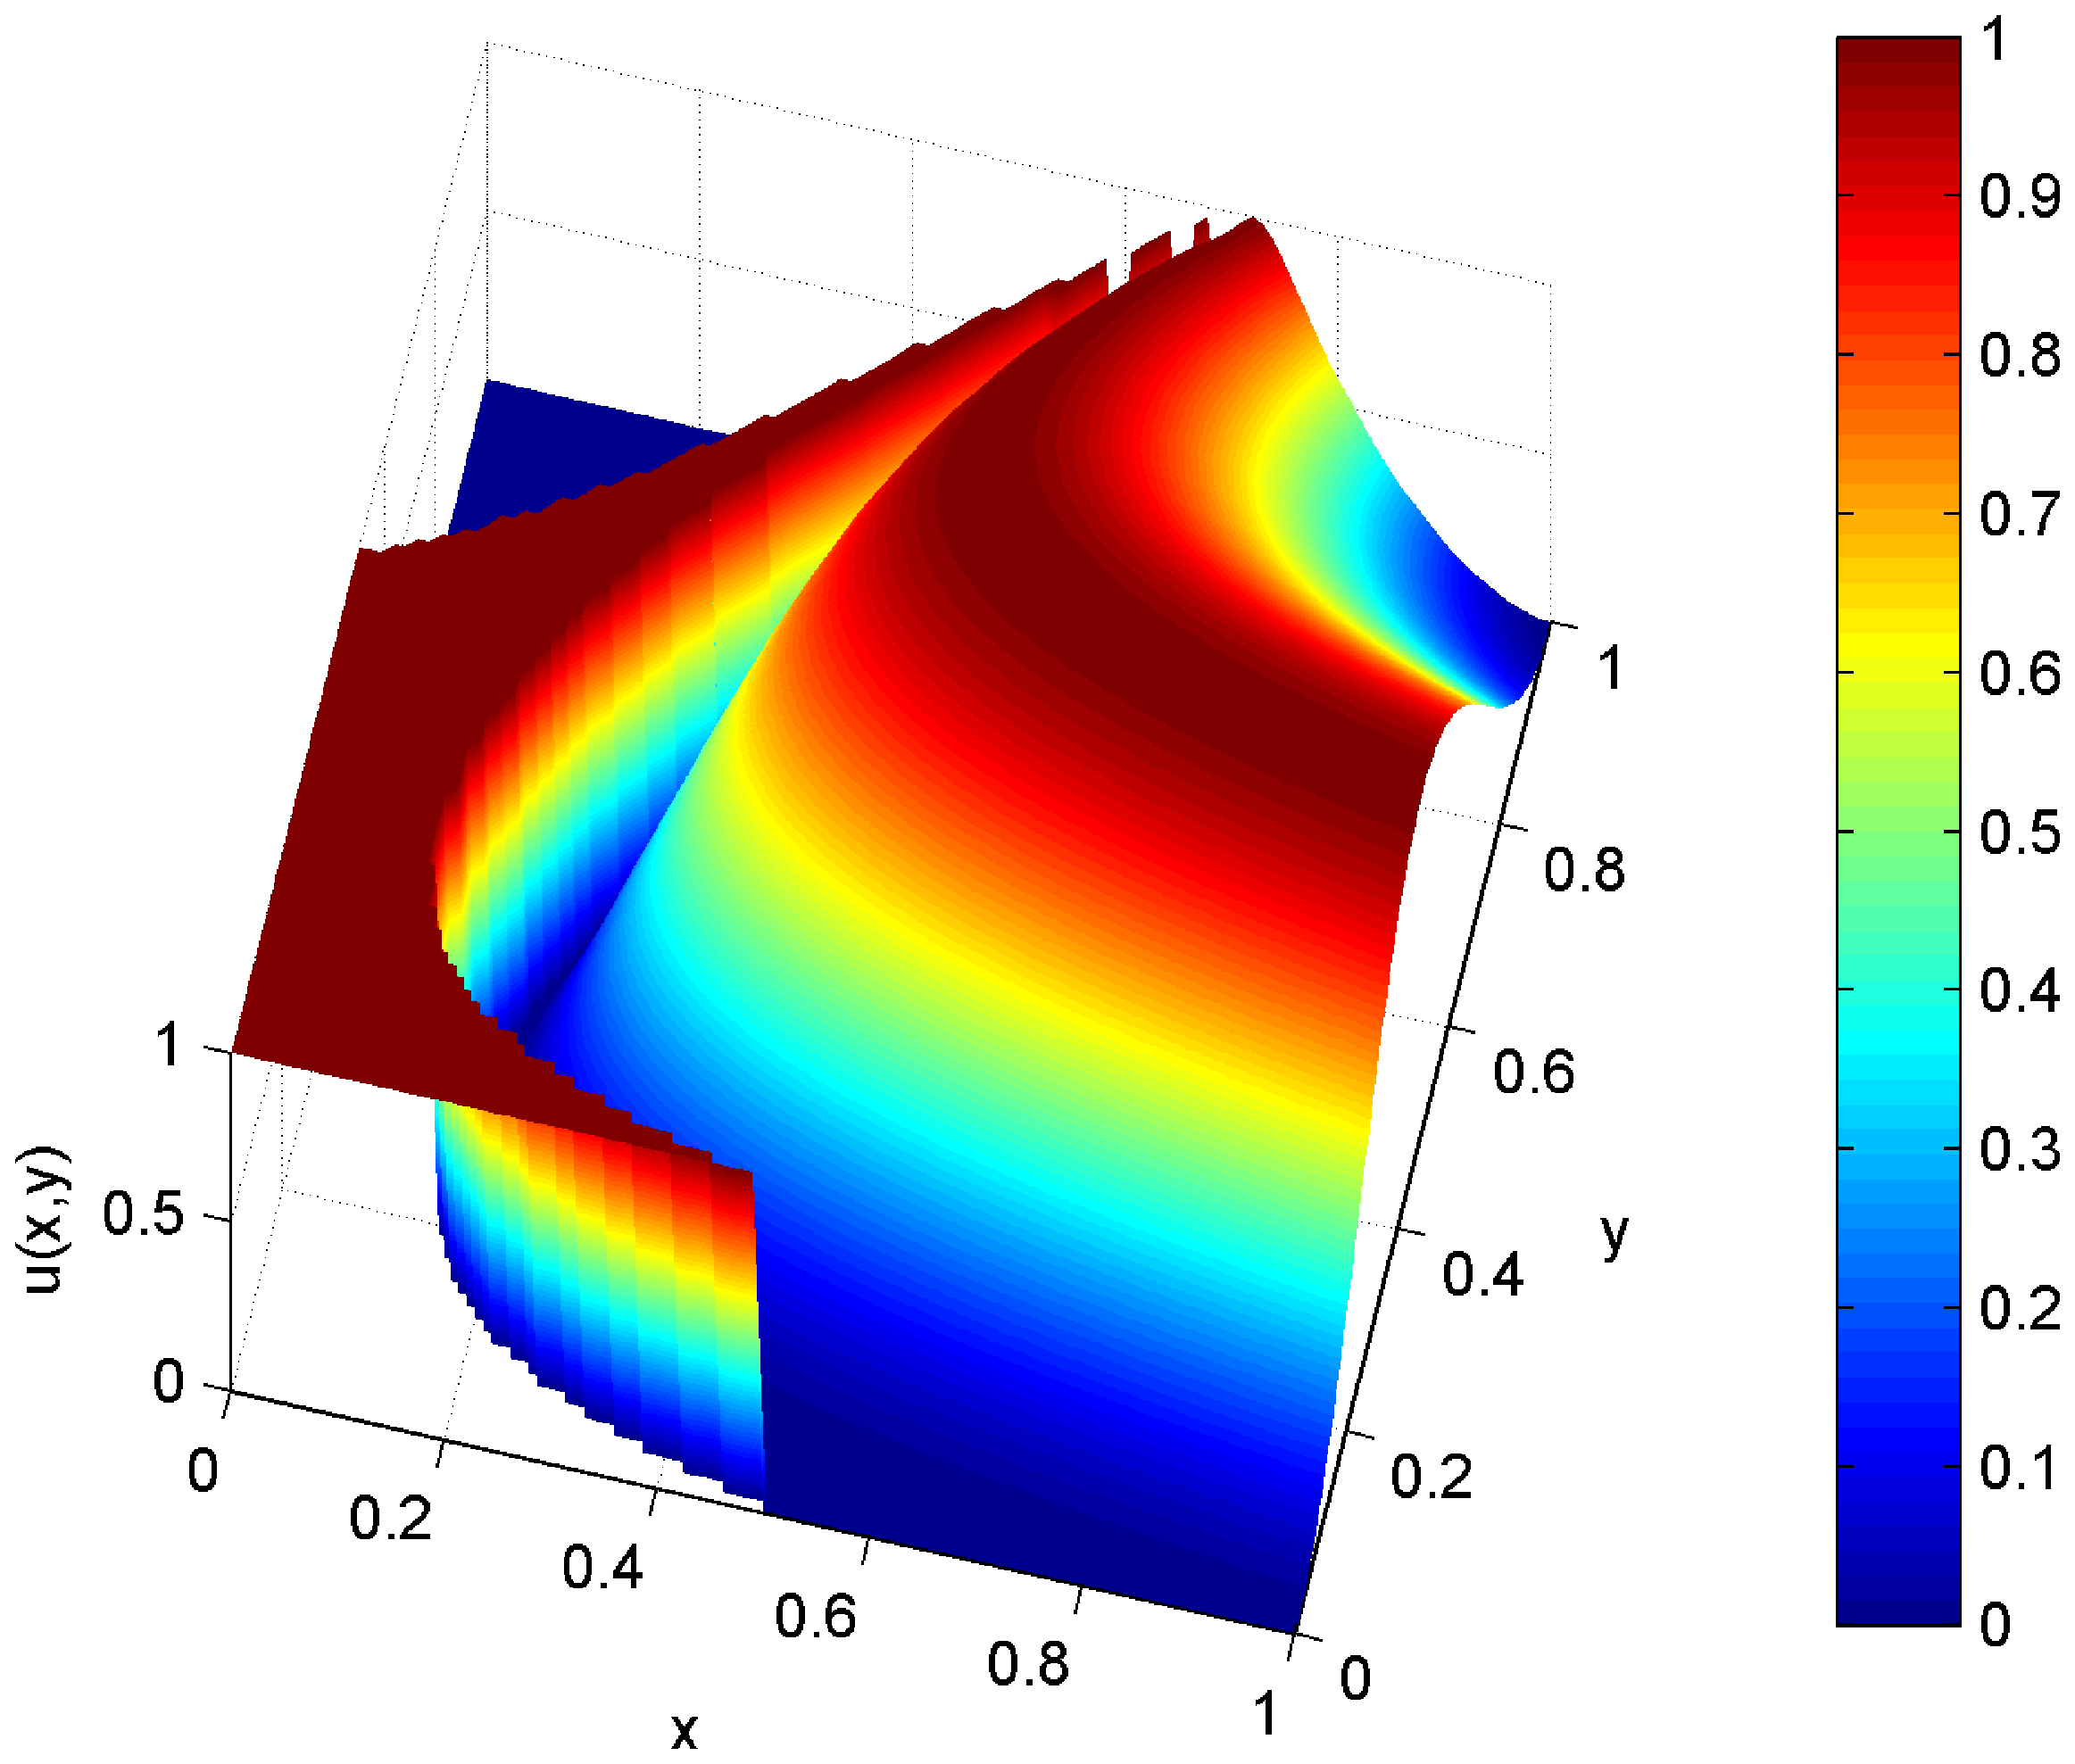
\includegraphics[scale=.14]{exact.eps}\hspace{1.5em}
    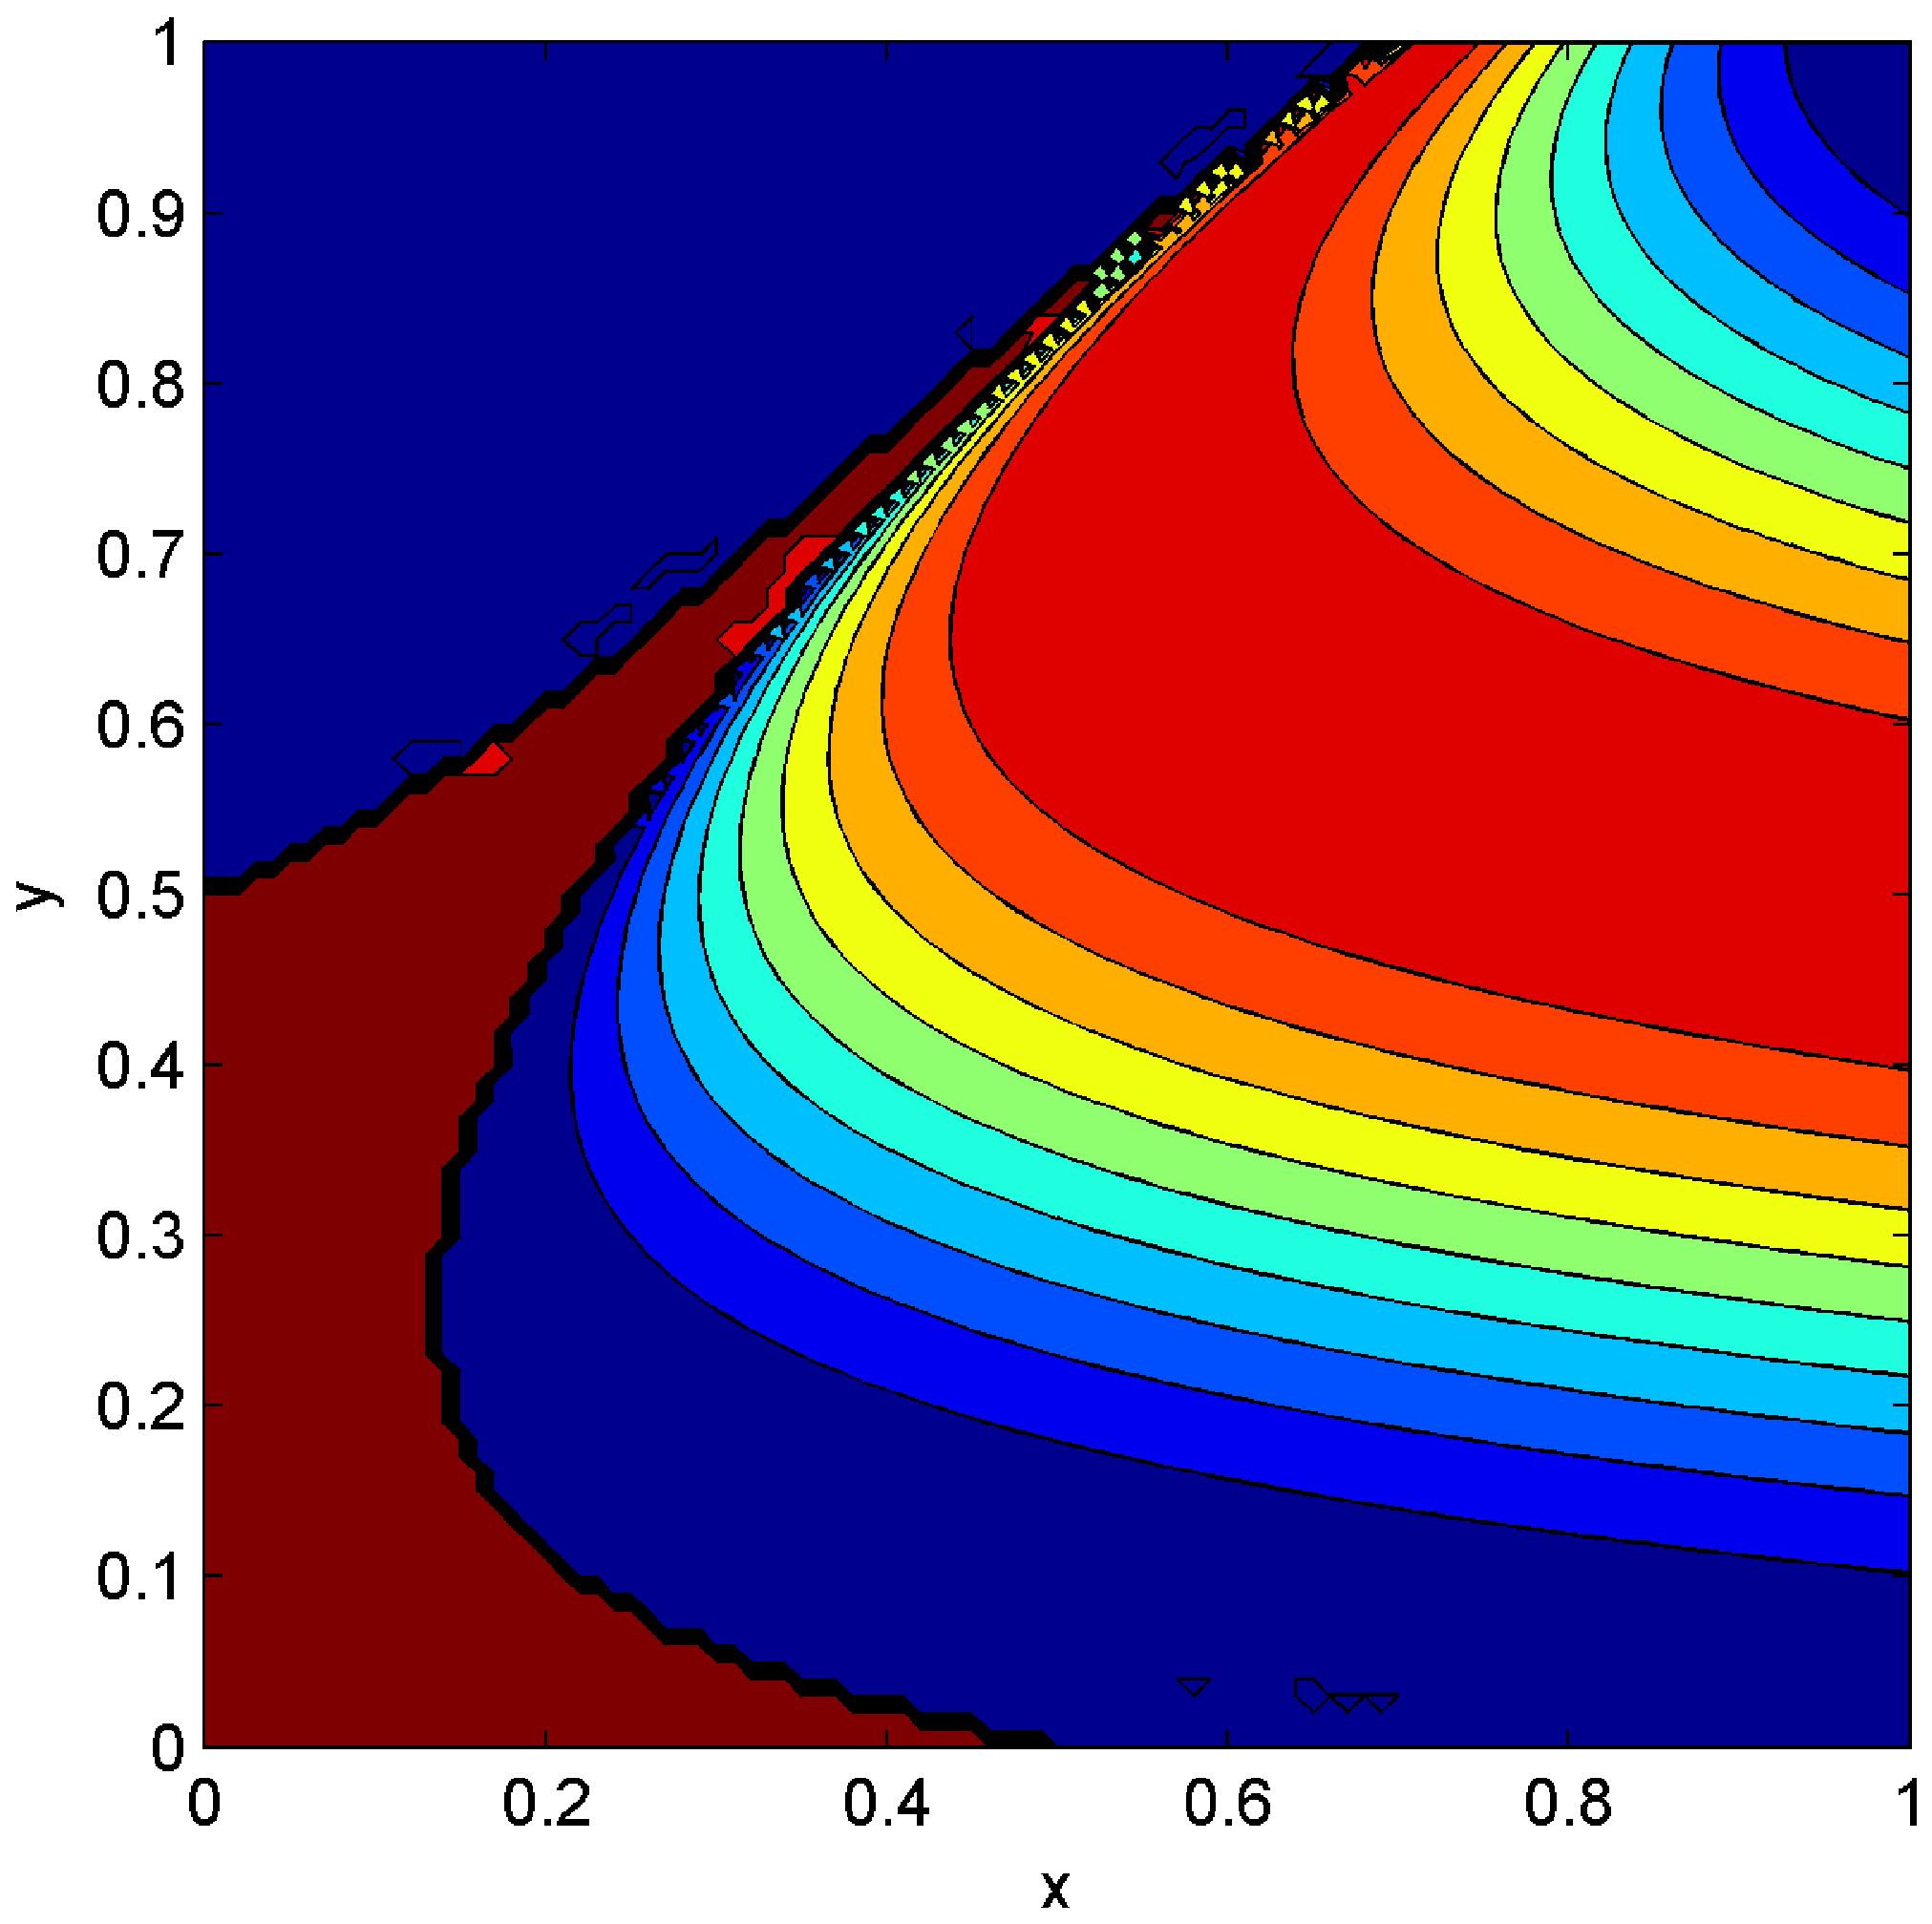
\includegraphics[scale=.12]{exactc.eps}    
    \caption{Přesné řešení vyhodnocené ve $100\times100$ bodech čtverce $\Omega$.}
    \label{fig:ref}
   \end{center}
  \end{figure}
\end{itemize}

\section{Metody konečných prvků (MKP)}
MKP, populární zejména pro řešení diferenciálních úloh druhého a vyššího řádu, nebyly zpočátku pro transportní výpočty příliš atraktivní. Předpokládají totiž hladkost řešení, kterou nelze obecně v případě parciálních diferenciálních rovnic hyperbolického typu očekávat. Průlom učinil až článek \cite{Reed}, v němž byla představena metoda nespojitých konečných prvků (\uv{Discontinuous Galerkin Method}, dále jen DGM). Přestože DGM umožňuje využít příznivé vlastnosti MKP (geometrická flexibilita, snadno použitelná aproximace vysokého řádu atd.) i pro úlohy s nehladkým řešením, její použití je obvykle spojeno s většími výpočetními nároky než u klasické MKP. Zároveň proto probíhal vývoj tzv. stabilizovaných metod konečných prvků (SMKP), v nichž je zachována globálně spojitá aproximace řešení a problémy s jeho nízkou regularitou jsou adresovány úpravami diskrétní formulace. 

DGM i SMKP využívají standardní rozklad (triangulaci)
$
  \overline\Omega = \cup_{K\in\tau_h}\overline K
$
oblasti $\Omega$ na množinu $\tau_h$ disjunktních elementů (v této práci čtverců) $K$ a přibližné řešení $u_h$ vyjadřují jako lineární kombinaci konečného počtu nad nimi definovaných bázových funkcí. Dosazením tohoto rozvoje do rovnice \eqref{eq:main} a aplikací Galerkinovy metody je původní spojitá úloha v obou případech převedena na řešení soustavy lineárních rovnic pro neznámé koeficienty rozvoje. Praktické provedení tohoto postupu a tvar výsledné soustavy se však pro oba typy metod liší.  

Z prostorových důvodů se zde budeme věnovat pouze nespojité Galerkinově metodě. Prostor bázových funkcí je pro ni definován jako 
$$
  V_{h} = \{v\in L^2(\Omega); v\vert_K\in P^p(K)\ \forall K\in \tau_h\},
$$
kde $P^p$ představuje prostor polynomů stupně nejvýše $p$ definovaných na elementu $K$. 
Klasický Galerkinův postup pro získání diskrétní verze dané úlohy vede v tomto případě (kdy je kvůli nedostatečné globální hladkosti funkcí z $V_{h}$ nutné pro použití Greenovy věty integrovat po elementech) k jejímu následujícímu znění:
Najdi $u_{h}\in V_{h}$ tak, aby $\forall v_{h}\in V_{h}$ platilo:
$$
\begin{gathered}
  \sumelem\intelem{(-u_h \afield\cdot \nabla v_h + c u_h v_h)} + \suminedge\intedge{\avg{\afield u_h}\cdot\jump{v_h}} = -\sumexedge\intedge{(\afield\cdot\bn)g v_h},\\[.3em]
  \avg{\afield u_h} =
  \begin{cases}
    \afield u_h^L, & \mbox{ když }\ \afield\cdot\bn^L > 0,\\[.25em]
    \afield u_h^R, & \mbox{ když }\ \afield\cdot\bn^L < 0,\\[.25em]
    \afield \frac{u_h^L + u_h^R}{2},\ & \mbox{ když } \afield\cdot\bn^L = 0,
   \end{cases}\quad
   \jump{v_h} = 
   \begin{cases}
    v_h\bn^L + v_h\bn^R & \mbox{ pro } e \not\subset\partial\Omega,\\[.25em]
    v_h\bn & \mbox{ pro } e \subset\partial\Omega,
   \end{cases}
\end{gathered}
$$
kde $e$ značí postupně hrany všech elementů $\tau_h$ a $L$, $R$ sousední elementy na jejich stranách.

Na funkce $v_{h}\in V_{h}$ se nekladou žádné požadavky z hlediska spojitosti mezi elementy a teoreticky ani z hlediska maximálního stupně $p$. To umožňuje relativně snadnou implementaci adaptivního zjemňování sítě (h-adaptivita) a zvyšování řádu aproximace (p-adaptivita) bez starosti o konformitu elementů. Předběžné výsledky adaptivního výpočtu jsou na obr. \ref{fig:subfigureExample}. Byla použita jednoduchá automatická adaptivita, řízená velikostí L2 normy rozdílu řešení na dané síti a jeho L2-projekce na globálně zhrubenou síť. Na obrázcích je patrná dostatečná schopnost h-adaptivity zachytit nespojitosti v řešení. Při použití elementů vyššího řádu je lépe aproximováno řešení na okolí nespojitosti blízko odtokové hrany, objevují se v něm však nerealistické oscilace a ukazuje se, že upwinding zahrnutý v definici $\avg{\cdot}$ zde sám o sobě k zaručení stability nestačí.

\begin{figure}[ht]
\centering
\subfigure[$p=0$, h-adapt. $\rightarrow$ 83680 NDOF]{
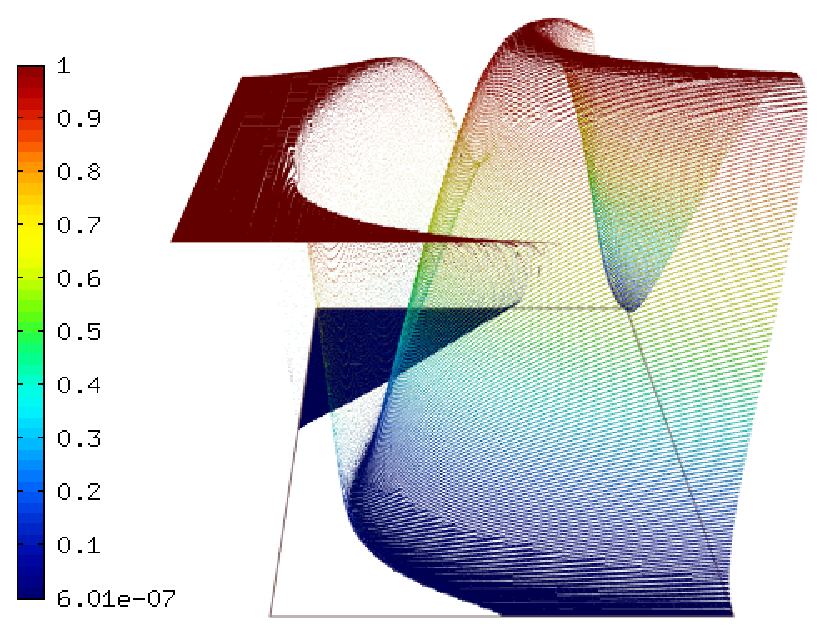
\includegraphics[scale=.30]{dg0.eps}\hspace{1em}
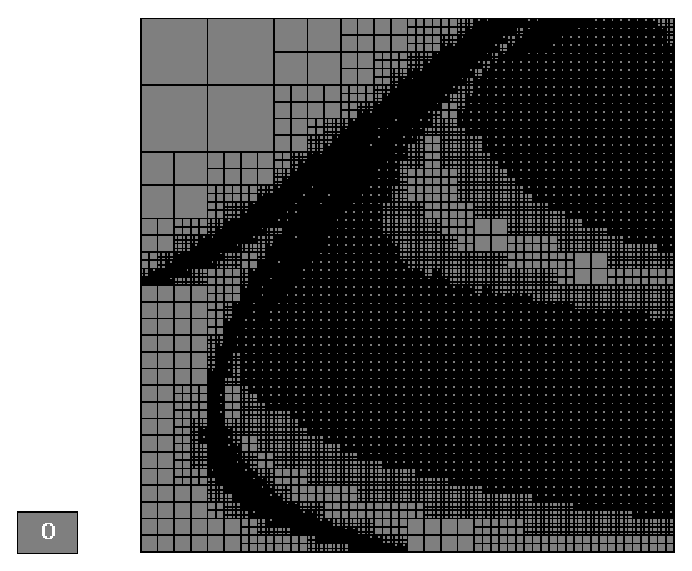
\includegraphics[scale=.30]{dg0-83680.eps}\hspace{1em}
\label{fig:dg1}
}
\subfigure[hp-adaptivita $\rightarrow$ 85220 NDOF]{
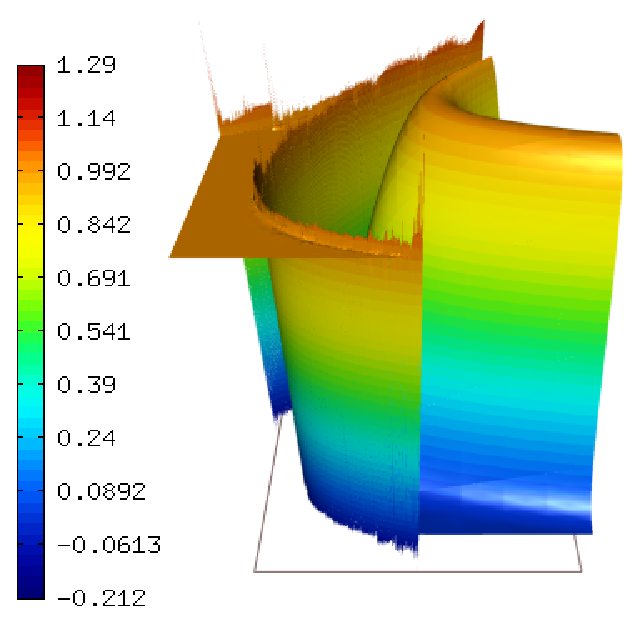
\includegraphics[scale=.30]{dg-hp.eps}\hspace{1em}
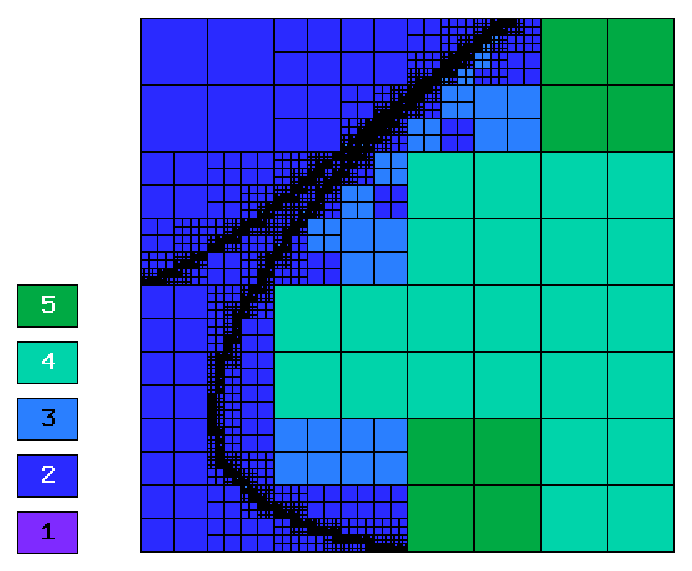
\includegraphics[scale=.30]{dg-hp-85220.eps}
\label{fig:dg3}
}
\caption[]{\parbox[t]{.9\textwidth}{Adaptivní DGM. NDOF $\ldots$ počet neznámých po konvergenci adaptačního procesu.\\ Čísla příslušná barvám elementů odpovídají řádu na nich def. bázových funkcí.}}
\label{fig:subfigureExample}
\end{figure}

\section{Residual distribution schemes (RDS)}
Další skupinou metod, jimž je v poslední době věnována značná pozornost, jsou metody typu RDS. Ty vznikly na základě myšlenek inspirovaných přístupy metody konečných objemů i MKP a přirozeně se snaží zachovat dobré vlastnosti obou. Z prvně jmenované tak např. robustnost danou silným vztahem k fyzikální podstatě řešeného problému, z druhé např. kompaktnost diskretizace i pro aproximaci vyššího řádu, jež umožňuje vývoj efektivních implicitních řešičů a jednoduchou paralelizaci (viz \cite{Deconinck-2003-IRD}).

Pro řešení testovací úlohy nestacionárním schématem typu RDS použijeme metodu ustalování. Pro nestacionární řešení vyššího řádu přesnosti v čase by bylo nutné použít konzistentní časovou diskretizaci, zde stačí nekonzistentní časová diskretizace (detaily viz \cite{Deconinck-2003-IRD}).

Uvažujme skalární zákon zachování $u_t+ \nabla \cdot (\mathbf{a}u) = 0$ a libovolnou triangulaci oblasti $\Omega$. Řešení je, obdobně jako v MKP 1. řádu, aproximováno spojitou funkcí lineární na každém trojúhelníku, $u(x,y,t)\approx\sum_i u_i(t)N_i(x,y)$, kde $u_i(t)$ je hodnota funkce $u$ v uzlu $i$ a $N_i$ jsou standardní P1 bázové funkce.

Definujeme reziduum na trojúhelníku $K$ jako 
\begin{equation*}
\phi^K=-\intelem{u_t}=\oint_{\partial K}(\overline{\mathbf{a}}u)\cdot\mathrm{d}\mathbf{n},\quad \mbox{ kde}\quad \overline{\mathbf{a}} = \frac{1}{K}\intelem{\mathbf{a}}.
\end{equation*}

Metoda RDS je založena na distribuci částí tohoto rezidua na sousední uzly. Vyjdeme-li z nekonzistentní formulace a Eulerovy explicitní integrace v čase, získáme následující schéma
\begin{equation*}
u_i^{n+1}=u_i^n-\frac{\Delta t}{S_i}\sum_T\beta^K_i\phi^K=u_i^n-\frac{\Delta t}{S_i}\sum_T\phi^K_i,
\end{equation*}
\begin{wrapfigure}{r}{.3\textwidth}
\begin{center}
\includegraphics{rds111.eps}
\caption{Geometrické znázornění základních prvků RDS.}
\end{center}
\end{wrapfigure}
kde $S_i$ je obsah  duální buňky okolo uzlu $i$, tj. 1/3 obsahu všech trojúhelníků se společným vrcholem v uzlu $i$. Pro daný trojúhelník požadujeme, aby \mbox{$\beta_1^K+\beta_2^K+\beta_3^K=1$} (konzervativita). Distribuční koeficienty $\beta$ mohou být stanoveny různými způsoby s ohledem na požadované vlastnosti monotónnosti a přesnosti řešení, kompaktní stencil zůstává zachován. Formálně definujeme distribuovaná rezidua jako \mbox{$\phi^K_i=\beta^K_i\phi^K$}.

Z metod typu RDS jsme vybrali N (Narrow) schéma s \mbox{$\phi_i^{K,N}=-\frac{k_i^+}{\sum_jk_j^+}\sum_jk_j^-(q_i^n-q_j^n)$} (monotónní lineární 1. řádu).
% a LDA (Low Diffusion A) schéma s $\beta_i^{LDA}=\frac{k_i^+}{\sum_jk_j^+}$ (lineární druhého řádu)
Čísla $k_i$, definovaná jako $k_i=\frac{1}{2}\mathbf{a}\cdot\mathbf{n}_i$, nám dovolují rozlišit mezi vtokovými a odtokovými stranami a vrcholy trojúhelníka. Vektory $\mathbf{n}_i$ jsou definované jako vnitřní normály trojúhelníku o velikosti rovné délce příslušné strany. Pro více informací viz \cite{Deconinck-2003-IRD}.

\begin{figure}[h]
  \begin{center}
    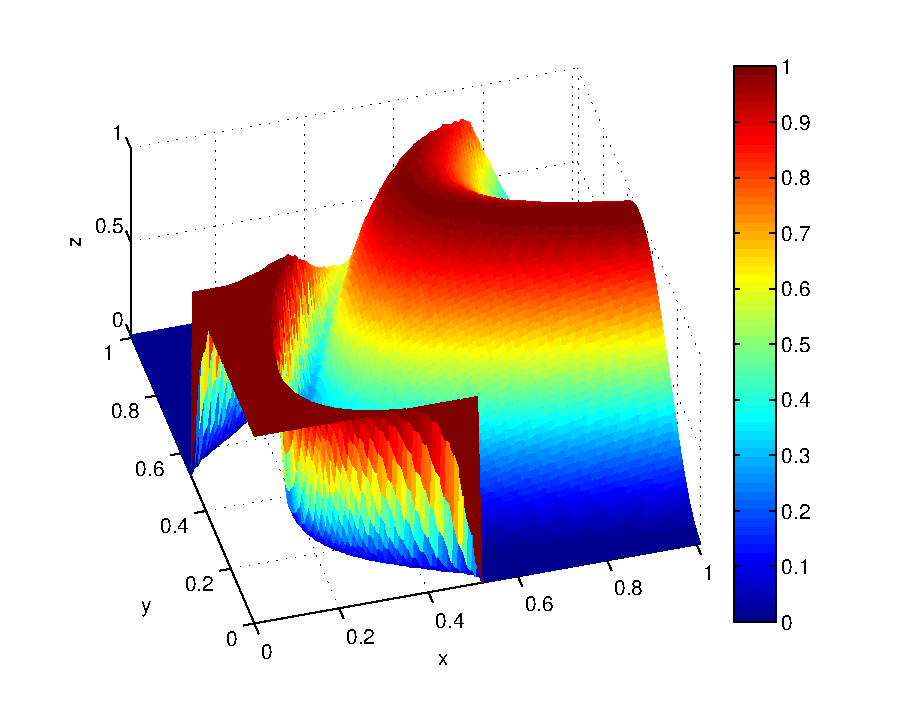
\includegraphics[width=6cm]{N_surf.eps}\hspace{2em}
    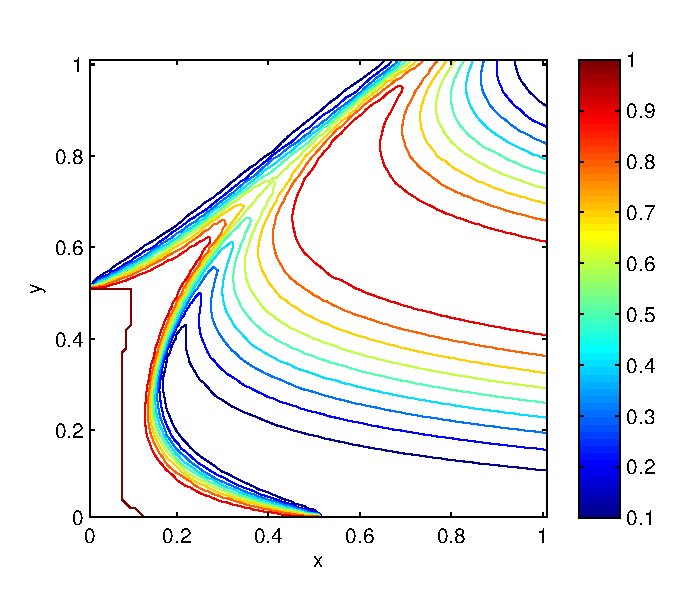
\includegraphics[width=5.5cm]{N_cont.eps}
  \caption{Numerické výsledky pro N schéma.}
  \label{fig:rds}
  \end{center}
  \end{figure}
  
\section{Závěr}
Předběžné výsledky prezentované výše slibují použitelnost RDS i DGM pro řešení netriviálních transportních úloh. Obě metody však mají své neduhy (patrné při porovnání obr. \ref{fig:subfigureExample} a \ref{fig:rds} s obr. \ref{fig:ref}, na jejichž odstranění autoři textu v současné době pracují. Na semináři pak budou RDS, DGM i SMKP důkladněji porovnány.

\begin{thebibliography}{m}

\bibitem{Deconinck-2003-IRD}
Deconinck H., Ricchiuto M., and Sermeus K.:
Introduction to residual distribution schemes and comparison with stabilized finite elements.
In: H. Deconinck (Ed.),
\emph{33rd VKI Lecture Series CFD}. Von
Karman Institute, Sint-Genesius-Rode, 2003.

\bibitem{Houston}
Houston P., Rannacher R., Süli E.:
A posteriori error analysis for stabilised finite element approximations of transport problems.
In: Comput. Methods Appl. Mech. Engrg. 190, 2000, pp. 1483--1508.

\bibitem{Reed}
Reed W. H., Hill T. R.: Triangular mesh methods for the neutron transport equation.
Tech. Report LA-UR-73-479,
Los Alamos Scientific Laboratory, 1973.

\end{thebibliography}

\end{document}
